%%%%%%%%%%%%%%%%%%%%%%%%%%%%%%%%%%%%%%%%%
% Wenneker Article
% LaTeX Template
% Version 2.0 (28/2/17)
%
% This template was downloaded from:
% http://www.LaTeXTemplates.com
%
% Authors:
% Vel (vel@LaTeXTemplates.com)
% Frits Wenneker
%
% License:
% CC BY-NC-SA 3.0 (http://creativecommons.org/licenses/by-nc-sa/3.0/)
%
%%%%%%%%%%%%%%%%%%%%%%%%%%%%%%%%%%%%%%%%%

%----------------------------------------------------------------------------------------
%	PACKAGES AND OTHER DOCUMENT CONFIGURATIONS
%----------------------------------------------------------------------------------------

\documentclass[10pt, a4paper, twocolumn]{article} % 10pt font size (11 and 12 also possible), A4 paper (letterpaper for US letter) and two column layout (remove for one column)

%%%%%%%%%%%%%%%%%%%%%%%%%%%%%%%%%%%%%%%%%
% Wenneker Article
% Structure Specification File
% Version 1.0 (28/2/17)
%
% This file originates from:
% http://www.LaTeXTemplates.com
%
% Authors:
% Frits Wenneker
% Vel (vel@LaTeXTemplates.com)
%
% License:
% CC BY-NC-SA 3.0 (http://creativecommons.org/licenses/by-nc-sa/3.0/)
%
%%%%%%%%%%%%%%%%%%%%%%%%%%%%%%%%%%%%%%%%%

%----------------------------------------------------------------------------------------
%	PACKAGES AND OTHER DOCUMENT CONFIGURATIONS
%----------------------------------------------------------------------------------------

\usepackage[english]{babel} % English language hyphenation

\usepackage{microtype} % Better typography

\usepackage{amsmath,amsfonts,amsthm} % Math packages for equations

\usepackage[svgnames]{xcolor} % Enabling colors by their 'svgnames'

\usepackage[hang, small, labelfont=bf, up, textfont=it]{caption} % Custom captions under/above tables and figures

\usepackage{booktabs} % Horizontal rules in tables

\usepackage{lastpage} % Used to determine the number of pages in the document (for "Page X of Total")

\usepackage{graphicx} % Required for adding images

\usepackage{enumitem} % Required for customising lists
\setlist{noitemsep} % Remove spacing between bullet/numbered list elements

\usepackage{sectsty} % Enables custom section titles
\allsectionsfont{\usefont{OT1}{phv}{b}{n}} % Change the font of all section commands (Helvetica)

%----------------------------------------------------------------------------------------
%	MARGINS AND SPACING
%----------------------------------------------------------------------------------------

\usepackage{geometry} % Required for adjusting page dimensions

\geometry{
	top=1cm, % Top margin
	bottom=1.5cm, % Bottom margin
	left=2cm, % Left margin
	right=2cm, % Right margin
	includehead, % Include space for a header
	includefoot, % Include space for a footer
	%showframe, % Uncomment to show how the type block is set on the page
}

\setlength{\columnsep}{7mm} % Column separation width

%----------------------------------------------------------------------------------------
%	FONTS
%----------------------------------------------------------------------------------------

\usepackage[T1]{fontenc} % Output font encoding for international characters
\usepackage[utf8]{inputenc} % Required for inputting international characters

\usepackage{XCharter} % Use the XCharter font

%----------------------------------------------------------------------------------------
%	HEADERS AND FOOTERS
%----------------------------------------------------------------------------------------

\usepackage{fancyhdr} % Needed to define custom headers/footers
\pagestyle{fancy} % Enables the custom headers/footers

\renewcommand{\headrulewidth}{0.0pt} % No header rule
\renewcommand{\footrulewidth}{0.4pt} % Thin footer rule

\renewcommand{\sectionmark}[1]{\markboth{#1}{}} % Removes the section number from the header when \leftmark is used

%\nouppercase\leftmark % Add this to one of the lines below if you want a section title in the header/footer

% Headers
\lhead{} % Left header
% \chead{\textit{\thetitle}} % Center header - currently printing the article title
\rhead{} % Right header

% Footers
\lfoot{} % Left footer
\cfoot{} % Center footer
\rfoot{\footnotesize Page \thepage\ of \pageref{LastPage}} % Right footer, "Page 1 of 2"

\fancypagestyle{firstpage}{ % Page style for the first page with the title
	% \fancyhf{}
	% \renewcommand{\footrulewidth}{0pt} % Suppress footer rule
}

%----------------------------------------------------------------------------------------
%	TITLE SECTION
%----------------------------------------------------------------------------------------

\newcommand{\authorstyle}[1]{{\large\usefont{OT1}{phv}{b}{n}\color{MidnightBlue}#1}} % Authors style (Helvetica)

\newcommand{\institution}[1]{{\footnotesize\usefont{OT1}{phv}{m}{sl}\color{MidnightBlue}#1}} % Institutions style (Helvetica)

\usepackage{titling} % Allows custom title configuration

\newcommand{\HorRule}{\color{MidnightBlue}\rule{\linewidth}{1pt}} % Defines the gold horizontal rule around the title

\pretitle{
	\vspace{-30pt} % Move the entire title section up
	\HorRule\vspace{10pt} % Horizontal rule before the title
	\fontsize{20}{25}\usefont{OT1}{phv}{b}{n}\selectfont % Helvetica
	\color{MidnightBlue} % Text colour for the title and author(s)
}

\posttitle{\par\vskip 1pt} % Whitespace under the title

\preauthor{} % Anything that will appear before \author is printed

\postauthor{ % Anything that will appear after \author is printed
	\vspace{10pt} % Space before the rule
	\par\HorRule % Horizontal rule after the title
	\vspace{20pt} % Space after the title section
}

%----------------------------------------------------------------------------------------
%	ABSTRACT
%----------------------------------------------------------------------------------------

\usepackage{lettrine} % Package to accentuate the first letter of the text (lettrine)
\usepackage{fix-cm}	% Fixes the height of the lettrine

\newcommand{\initial}[1]{ % Defines the command and style for the lettrine
	\lettrine[lines=3,findent=4pt,nindent=0pt]{% Lettrine takes up 3 lines, the text to the right of it is indented 4pt and further indenting of lines 2+ is stopped
		\color{MidnightBlue}% Lettrine colour
		{#1}% The letter
	}{}%
}

\usepackage{xstring} % Required for string manipulation

\newcommand{\lettrineabstract}[1]{
	\StrLeft{#1}{1}[\firstletter] % Capture the first letter of the abstract for the lettrine
	\initial{\firstletter}\textbf{\StrGobbleLeft{#1}{1}} % Print the abstract with the first letter as a lettrine and the rest in bold
}

%----------------------------------------------------------------------------------------
%	BIBLIOGRAPHY
%----------------------------------------------------------------------------------------

\usepackage[backend=bibtex,style=authoryear,natbib=true]{biblatex} % Use the bibtex backend with the authoryear citation style (which resembles APA)

\addbibresource{example.bib} % The filename of the bibliography

\usepackage[autostyle=true]{csquotes} % Required to generate language-dependent quotes in the bibliography
 % Specifies the document structure and loads requires packages
\usepackage{hyperref}
\hypersetup{
  colorlinks = true,
  urlcolor   = blue,
  linkcolor  = blue,
  citecolor  = red
}
\usepackage{graphicx}

%----------------------------------------------------------------------------------------
%	ARTICLE INFORMATION
%----------------------------------------------------------------------------------------

\title{COVID-19 project: graph mining and topic modeling} % The article title

\author{
	\authorstyle{Sebastiaan Van den Broeck} % Authors
}

\date{18/08/2022} % Add a date here if you would like one to appear underneath the title block, use \today for the current date, leave empty for no date

%----------------------------------------------------------------------------------------

\begin{document}

\maketitle % Print the title

\thispagestyle{firstpage} % Apply the page style for the first page (no headers and footers)

%----------------------------------------------------------------------------------------
%	ABSTRACT
%----------------------------------------------------------------------------------------

% TODO: add that all and more information can be found in the notebook

\lettrineabstract{There is no doubt about the enormous impact of COVID-19 on our world. That is to say, it is one of the most disastrous events of our lifetime yet. Despite the critical importance of this information, not much is known about it. The information has become wrapped up in politics and misinformation. The appearance of a pandemic is a random event. It is therefore not possible to predict when the next one will occur. However, it is a safe assumption that one will happen again in the future. Any information we can uncover now can surely be of use later (Relman, 2020). To that end, a data-driven analysis has been applied.}

%----------------------------------------------------------------------------------------
%	ARTICLE CONTENTS
%----------------------------------------------------------------------------------------

\section{Methodology}

\begin{figure}[h]
  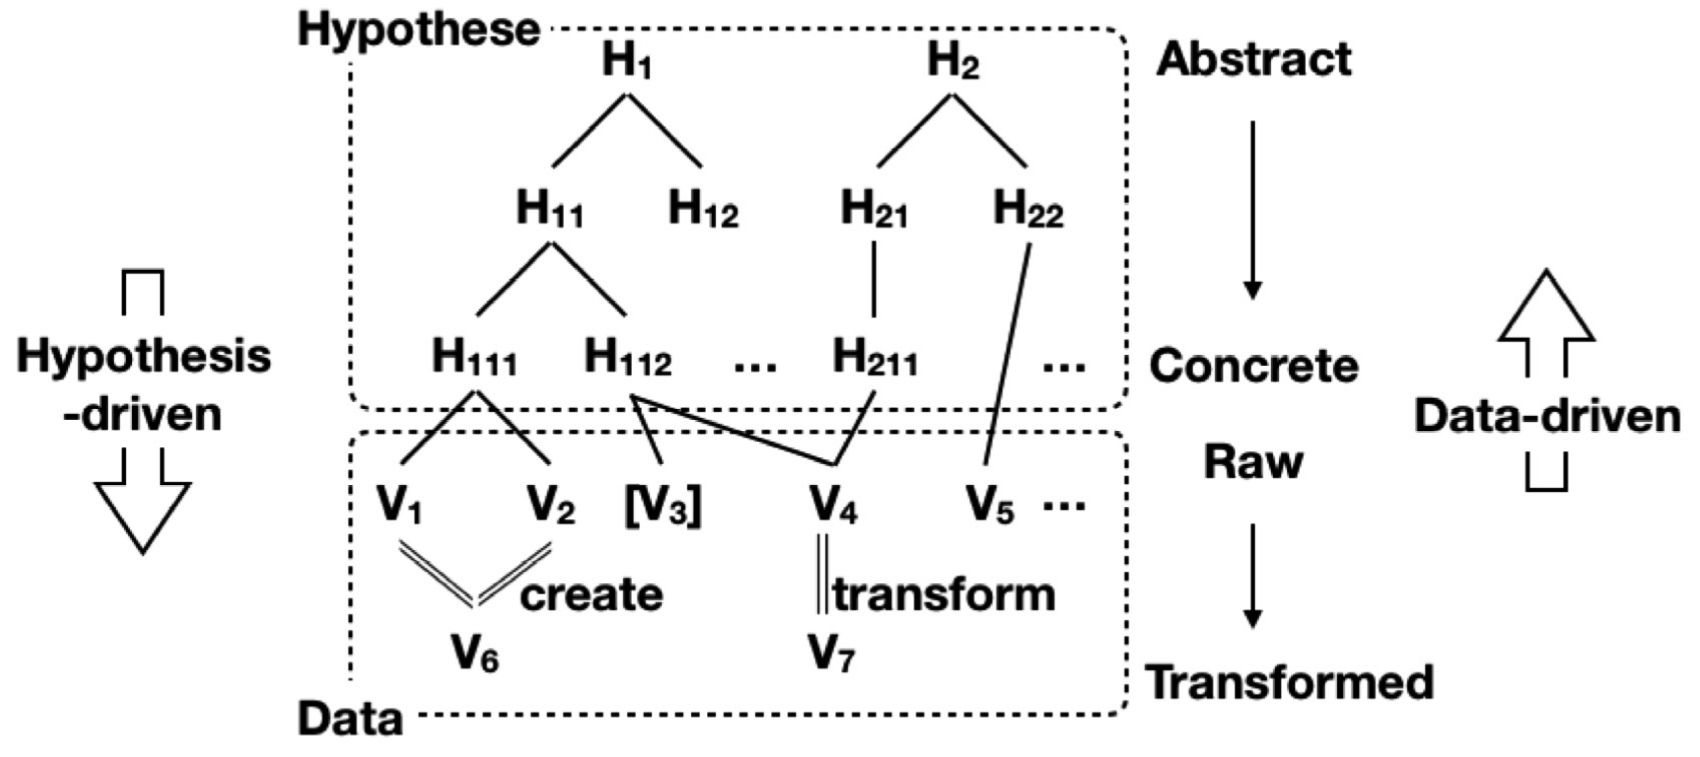
\includegraphics[width=\linewidth]{../visualizations/hypothesis_space_data_space.png}
  \caption{The relationship between the hypothesis space, data space, a hypothesis-driven analysis and a data-driven analysis. Taken from Matsumuro \& Miwa (2019).}
  \label{fig:topic_modelling}
\end{figure}

The scientific process can be described as a search in one of two spaces.
On the one hand, there exists the well-known hypothesis space. It contains all hypothesis that are organized from abstract to specific. First, the researcher will select a general hypothesis ($H_1$). Next, a more specific hypothesis will have to be formulated ($H_{111}$). Afterwards, the researcher can reach the variables contained in the data space. This method therefore has a high depth. It can start from a very general hypothesis and reach specific variables.

On the other hand, the data space has gotten more attention recently, because of a higher availability of data. It contains all relevant information with respect to the analysis. This method therefore has a wide reach, but not a lot of depth. A sound understanding of the data is therefore needed to analyze it. To that end, plots and tables have been used to visualize the data. However, datasets often contain inconsistencies and noise. It is therefore paramount to any data science undertaking to clean the data (Sarker, 2021).
The problem with a hypothesis-driven analysis has now become more clear. The researchers can only select one hypothesis (for example, $H_{111}$) and reach only a specific amount of variables. However, much more information is available in the data space. The data-driven analysis, then, tries to exploit this by including as much of the data space as possible. The question that remains is how one should reach a relevant hypothesis from the data (Matsumuro \& Miwa, 2019).

%------------------------------------------------

\section{Data sources}

Before starting the analysis we will discuss the data. The data treated in this report comes from various sources. First, there is the \href{https://github.com/nytimes/covid-19-data}{COVID-19 dataset} (The New York Times, 2021). The report takes a data-driven approach instead of a traditional hypothesis-driven approach. This dataset therefore fulfills a principal, directional role. It provides information on the number of cases on the national level, state level and county level in the United States. Moreover, there is information on mask use and the number of cases in prisons and colleges. 
Second, the previous dataset has been complemented with \href{https://apps.bea.gov/regional/downloadzip.cfm}{economical information} (Bureau of Economic Analysis, 2022). It provides information on the GDP of each state per industry. The information will allow us to not only examine the human impact of the pandemic, but also take a closer look at the economical impact.
Third, there is no doubt air transportation has played an important role in the pandemic. \href{https://zenodo.org/record/6411336\#.YmO_gS8RrzU}{The crowdsourced air traffic dataset} has therefore been added to the analysis (Strohmeier et al., 2021). It is a transformed and cleaned version from the OpenSky dataset and contains important information regarding the development of air traffic before and during the pandemic.
Fourth, \href{https://github.com/allenai/cord19}{the CORD-19 dataset} has been added to the analysis (Lucy et al., 2020). It contains a collection of more than 140000 scientific papers and related research.
%------------------------------------------------

\section{Graph mining}

The second part of the project has been devoted to graph mining. Graph mining is a general term that means mining information from a dataset that is represented by a graph structure (Rehman et al., 2012). In other words, the data is represented by nodes, relationships and properties. We will tap into a new part of the data space in the hopes of reaching an interesting hypothesis. To that end, different data sources can be combined. Modelling the spread of a disease using a graph approach is not new concept. For example, Manriquez et al. (2021) used an edge-weighted graph to study the dissemination of an epidemic. Specifically, centrality measures have been used to find out the importance of airports. To that end, Neo4J can be used as a graph database. We can consider the airports as nodes and the flights as relationships between the airports. Moreover, an object-oriented programming approach has been taken.

The identification of which nodes in a network are the most important has been an important issue in network analysis (Opsahl et al., 2010). Indeed, different interpretations of "importance" will lead to different approaches.
To that end, three important interpretations of centrality have been formulated. First, the centrality of a node depends on the connectedness through immediate connections to other nodes. Second, the centrality of a node depends on the frequency with which the node falls on paths between other nodes. Third, the centrality of a graph depends on the degree to which it is close to the rest of the graph (Klein, 2010).
The first interpretation corresponds to the degree centrality. This metric tries to assess the importance of a node using the number of direct connections it has to other nodes. Within the context of our analysis it is certainly important to know how many connections an airport has to other ones. However, this centrality measure does not take into account the global structure of the network, but only the direct connections.
The second interpretation denotes the betweenness of a node. The betweenness centrality measures the extent to which a node lies on the shortest path between other nodes. There is no doubt that this interpretation is also important for our analysis.
The third interpretation is called the closeness centrality. It simply measures the inverse sum of the shortest distances to all the other nodes. However, we are not working with a weighted graph. The distance metric is therefore simply the number of hops between two airports. The interpretation after calculating this metric may be difficult. Another interesting approach could be constructing a graph where the weights are the distances between airports (Opsahl et al., 2020).

\begin{figure}[h]
  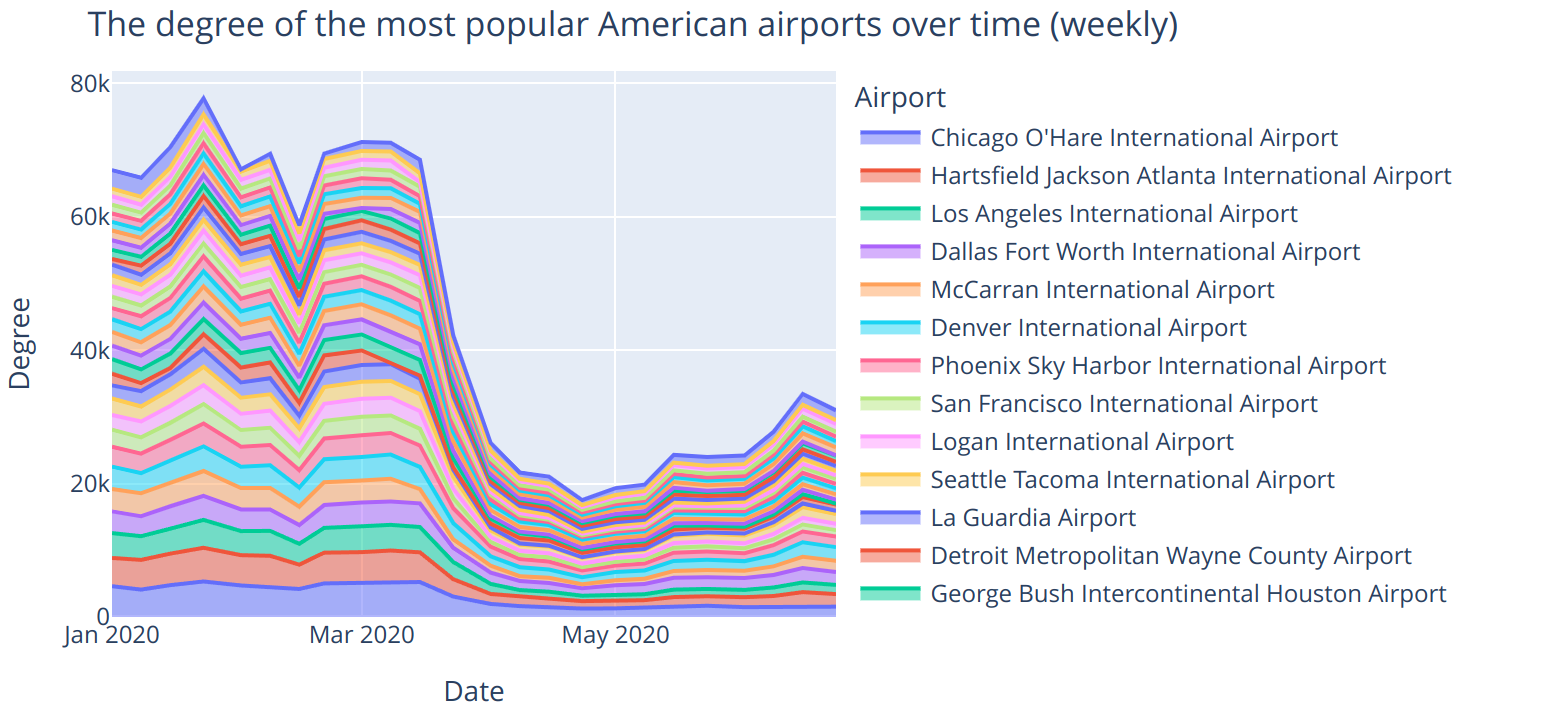
\includegraphics[width=\linewidth]{../visualizations/degree_screenshot.png}
  \caption{The degree of the most popular American airports took a sharp dive after the WHO declared COVID-19 a pandemic and after Trump declared a national emergency.}
  \label{fig:degree}
\end{figure}

\begin{figure}[h]
  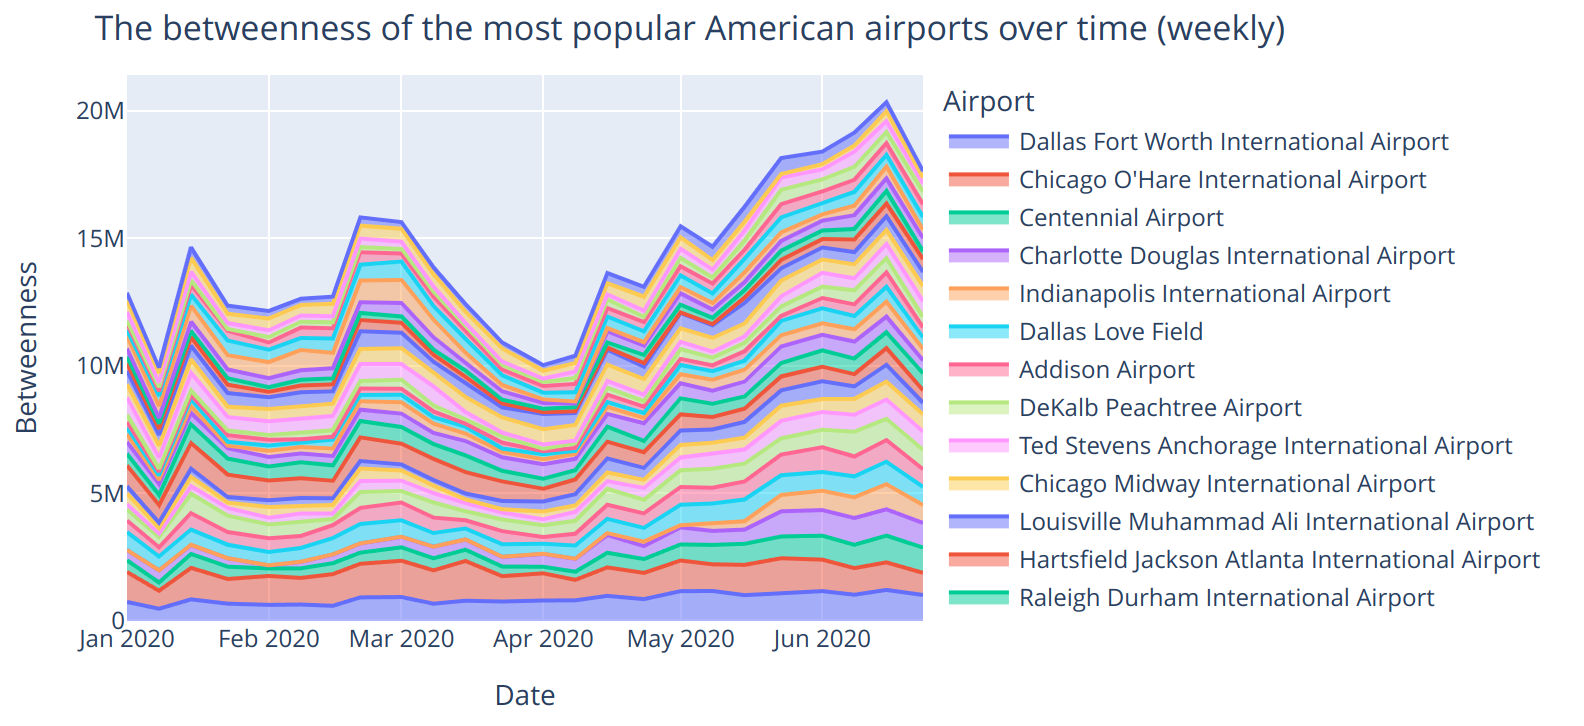
\includegraphics[width=\linewidth]{../visualizations/betweenness_screenshot.png}
  \caption{A similar trend can be detected for the betweenness centrality of American airports.}
  \label{fig:betweenness}
\end{figure}

%------------------------------------------------

\section{Text mining}

\begin{figure}[h]
  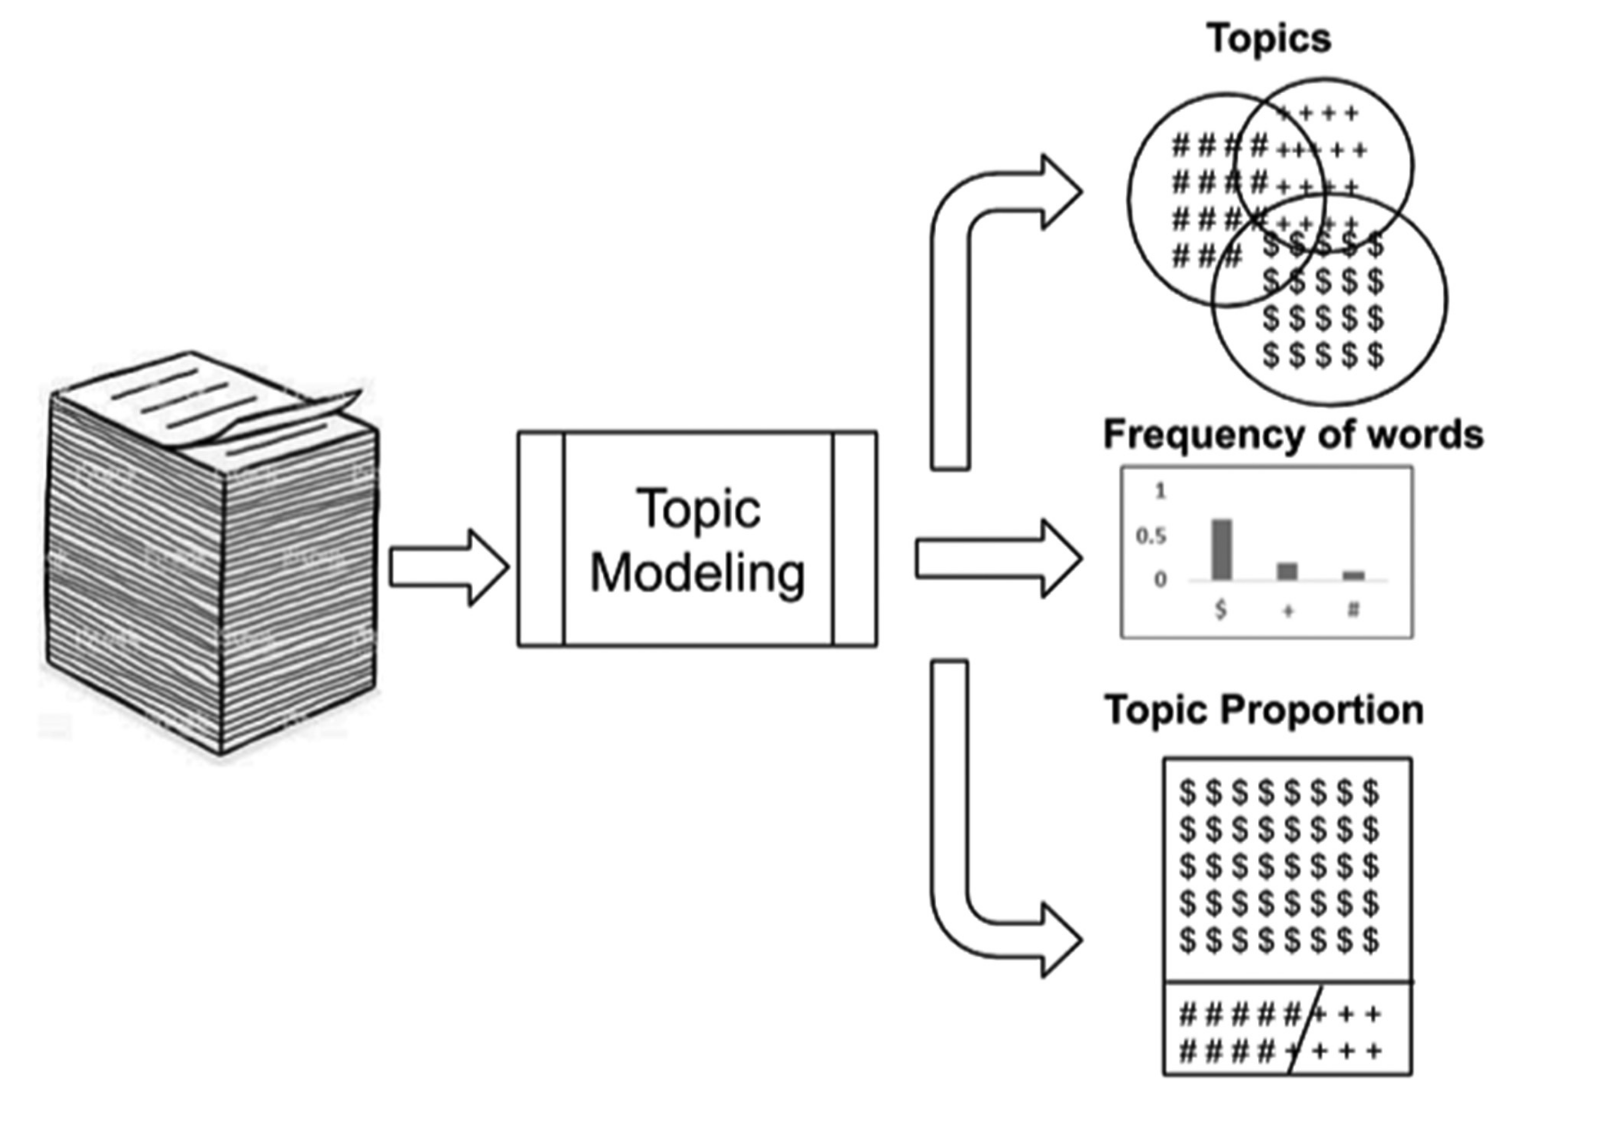
\includegraphics[width=\linewidth]{../visualizations/topic_modelling.png}
  \caption{The area of topic modelling is concerned with making inferences from a huge collection of documents in terms of topics, frequency of words and topic proportions. Taken from Chauchan \& Shah (2022).}
  \label{fig:topic_modelling}
\end{figure}

Third, another non-tabular data source that often goes unnoticed is text. Indeed, natural language processing, or text mining, is a family of techniques that tries to extract meaning from text documents. Topic modelling is one area of NLP that can be used to provide an overview from a very large collection of documents. Topic models, then, are statistical models that can be used to show the hidden structure of text data. In other words, they learn the latent semantic structures of a collection of text documents (Chauhan \& Shah, 2022).
The technique allows inferences to be made in terms of the whole collection, individual documents or relationships between the documents. Specifically, latent dirichlet allocation will be applied. The technique models a topic by word probabilities. Therefore, one can look at the words with the highest probabilities for each topic to get an idea of what the topic is about (Jelodar et al., 2019).

The dataset at hand is the COVID-19 open research dataset (CORD-19). It provides a collection of more than 140000 scientific papers and related research. The goal of the dataset is to use machine learning to discover relevant information. Therefore, it has been specifically designed for text mining purposes. However, limited preprocessing of the text has been done. We will therefore go through these steps ourselves (Lucy et al., 2020).

\begin{table}[h]
\caption{Topics before pandemic}
\centering
\scalebox{0.45}{
\begin{tabular}{|l|l|l|l|l|l|l|l|l|l|}
\hline
\textbf{Topic 1} & \textbf{Topic 2} & \textbf{Topic 3} & \textbf{Topic 4} & \textbf{Topic 5} & \textbf{Topic 6} & \textbf{Topic 7} & \textbf{Topic 8} & \textbf{Topic 9} & \textbf{Topic 10} \\ \hline
cell             & health           & patient          & cov              & cell             & infect           & immun            & vaccin           & calv             & der               \\ \hline
protein          & diseas           & respiratori      & detect           & protein          & respiratori      & vaccin           & viru             & protein          & die               \\ \hline
viru             & develop          & studi            & viru             & activ            & viral            & cell             & infect           & viru             & und               \\ \hline
viral            & model            & infect           & sequenc          & lung             & group            & respons          & influenza        & structur         & model             \\ \hline
infect           & public           & associ           & human            & express          & studi            & protein          & studi            & studi            & ein               \\ \hline
activ            & emerg            & children         & respiratori      & induc            & viru             & antigen          & result           & result           & network           \\ \hline
express          & data             & clinic           & virus            & airwai           & associ           & antibodi         & ibv              & effect           & von               \\ \hline
rna              & infecti          & influenza        & pcr              & result           & virus            & specif           & virus            & test             & mit               \\ \hline
virus            & studi            & case             & infect           & increas          & caus             & express          & protect          & differ           & bei               \\ \hline
host             & risk             & hospit           & sars             & mice             & patient          & infect           & effect           & domain           & cell              \\ \hline
\end{tabular}}
\end{table}

Next, we will look at the clusters of documents before and during the pandemic. A more detailed analysis has been given in the notebook. The table shown above denotes the 10 most important words per topic before the pandemic. 
First, we may notice that some improvements can still be made in the preprocessing of the documents. For example, the words \textit{viru}, \textit{viral} and \textit{virus} all mean the same thing. They should therefore be stemmed in a way that they become one token. Another problem becomes apparent when taking a closer look at topic 10. Apparently, one or more German papers have made their way into the dataset and have formed their own cluster. This may actually indicate that the LDA is working well, since these papers should clearly be in a cluster of their own.
Second, inferences can be made regarding the research itself. On the one hand, we can detect some clusters that have to do with the inner workings of the disease. For example, for the topic 1 and 5 the words \textit{cell}, \textit{protein} and \textit{rna} are important. On the other hand, some other topics appear to deal with the patient and the sociatal impact. For example, the words \textit{health}, \textit{disease}, \textit{public} and \textit{model} are important for topic 2. Topic 3, then, has the words \textit{patient}, \textit{respiratori} and \textit{studi} associated with it. It is also interesting to note that there is a cluster of documents that deals with vaccination. Topic 8 has the words \textit{vaccin}, \textit{infect} and \textit{influenza} associated with it.

\begin{table}[h]
\caption{Topics during pandemic}
\scalebox{0.45}{
\begin{tabular}{|l|l|l|l|l|l|l|l|l|l|}
\hline
\textbf{Topic 1} & \textbf{Topic 2} & \textbf{Topic 3} & \textbf{Topic 4} & \textbf{Topic 5} & \textbf{Topic 6} & \textbf{Topic 7} & \textbf{Topic 8} & \textbf{Topic 9} & \textbf{Topic 10} \\ \hline
health           & patient          & covid            & test             & patient          & cov              & protein          & health           & mask             & der               \\ \hline
covid            & covid            & model            & covid            & cell             & sars             & cov              & studi            & effect           & die               \\ \hline
studi            & hospit           & vaccin           & model            & covid            & covid            & cell             & mental           & covid            & und               \\ \hline
research         & risk             & case             & data             & diseas           & infect           & sars             & depress          & cov              & text              \\ \hline
data             & studi            & studi            & method           & treatment        & patient          & ace              & associ           & sars             & studi             \\ \hline
care             & clinic           & infect           & detect           & immun            & antibodi         & viral            & anxieti          & aerosol          & infect            \\ \hline
pandem           & sever            & number           & perform          & activ            & respiratori      & bind             & women            & patient          & activ             \\ \hline
provid           & associ           & effect           & result           & studi            & coronaviru       & covid            & social           & studi            & gene              \\ \hline
develop          & group            & data             & studi            & clinic           & sever            & viru             & covid            & infect           & effect            \\ \hline
social           & patients         & time             & sampl            & associ           & studi            & drug             & effect           & risk             & model             \\ \hline
\end{tabular}}
\end{table}

Next, we will take a look at the interpretation of the LDA that is trained on documents from after the start of the pandemic.
First, we may notice that there is a new cluster compared to the previous model. Cluster 9 has the words \textit{mask}, \textit{effect} and \textit{aerosol} associated with it. In other words, this is a cluster about the effectiveness of masks for the spread of COVID-19.
Second, there is again a cluster with German words. This gives an indication that still some work can be done on the preprocessing steps. On the other hand, it can indicate that the LDA is working well, because it can isolate this cluster.
Third, it is clear that the word \textit{covid} appears a lot in the clusters and is not very informative. It could therefore be removed in the preprocessing steps. More interpretation regarding the topics and their relationships to each other has been given in the notebook.

\section{Conclusion}

In this paper I have provided a fresh perspective on the COVID-19 pandemic. First, the New York Times COVID-19 dataset was used as the guiding force. In other words, it played a very important role in the exploratory data analysis. Second, economical information was used to provide more robust explanations. Third, the COVID-19 OpenSky dataset was used for graph mining. Fourth, the CORD-19 dataset was added to the mix to perform topic modelling.
The results of the analysis indicate a detrimental effect on all centrality measures of the airport-flights graph. We uncovered a sharp drop in the degree centrality after the WHO declared COVID-19 a pandemic and after Trump declared COVID-19 a national emergency. Moreover, we took a look at the locations of international airports and first COVID-19 cases. As could be expected, the locations of international airports are close to the first COVID-19 cases.
Second, text mining was applied to detect the change in scientific literature before and after the pandemic. The results indicate a higher importance of the treatment of individuals, vaccination and the effectiveness of masks.

\hspace{20px}

\hspace{20px}

\hspace{20px}

\hspace{20px}

\hspace{20px}

\hspace{20px}

\hspace{20px}

\hspace{20px}

\hspace{20px}

\hspace{20px}

\hspace{20px}

\pagebreak
\section{Bibliography}

\hspace{5px} Brandes, U. (2008). On variants of shortest-path betweenness centrality and their generic computation. Social Networks, 30(2), 136–145. \url{https://doi.org/10.1016/j.socnet.2007.11.001} \\

\vspace{-13px}

Bureau of Economic Analysis. (2022). Annual GDP per state [Dataset]. \url{https://apps.bea.gov/regional/downloadzip.cfm}

Chauhan, U., \& Shah, A. (2022). Topic Modeling Using Latent Dirichlet allocation: A Survey. ACM Computing Surveys, 54(7), 1–35. https://doi.org/10.1145/3462478

Jelodar, H., Wang, Y., Yuan, C., Feng, X., Jiang, X., Li, Y., \& Zhao, L. (2019). Latent Dirichlet allocation (LDA) and topic modeling: Models, applications, a survey. Multimedia Tools and Applications, 78(11), 15169–15211. \url{https://doi.org/10.1007/s11042-018-6894-4}

Klein, D. J. (2010). Centrality measure in graphs. Journal of Mathematical Chemistry, 47(4), 1209–1223. \url{https://doi.org/10.1007/s10910-009-9635-0}
 
Lucy Lu Wang, Kyle Lo, Yoganand Chandrasekhar, Russell Reas, Jiangjiang Yang, Doug Burdick, Darrin Eide, Kathryn Funk, Yannis Katsis, Rodney Michael Kinney, Yunyao Li, Ziyang Liu, William Merrill, Paul Mooney, Dewey A. Murdick, Devvret Rishi, Jerry Sheehan, Zhihong Shen, Brandon Stilson, et al.. 2020. CORD-19: The COVID-19 Open Research Dataset. In Proceedings of the 1st Workshop on NLP for COVID-19 at ACL 2020, Online. Association for Computational Linguistics.

Manríquez, R., Guerrero-Nancuante, C., Martínez, F., \& Taramasco, C. (2021). Spread of Epidemic Disease on Edge-Weighted Graphs from a Database: A Case Study of COVID-19. International Journal of Environmental Research and Public Health, 18(9), 4432. \url{https://doi.org/10.3390/ijerph18094432}

Matsumuro, M., \& Miwa, K. (2019). Model for Data Analysis Process and Its Relationship to the Hypothesis-Driven and Data-Driven Research Approaches. In A. Coy, Y. Hayashi, \& M. Chang (Eds.), Intelligent Tutoring Systems (Vol. 11528, pp. 123–132). Springer International Publishing. \url{https://doi.org/10.1007/978-3-030-22244-4_16}

Opsahl, T., Agneessens, F., \& Skvoretz, J. (2010). Node centrality in weighted networks: Generalizing degree and shortest paths. Social Networks, 32(3), 245–251. \url{https://doi.org/10.1016/j.socnet.2010.03.006}

Rehman, S. U., Khan, A. U., \& Fong, S. (2012). Graph mining: A survey of graph mining techniques. Seventh International Conference on Digital Information Management (ICDIM 2012), 88–92. \url{https://doi.org/10.1109/ICDIM.2012.6360146}

Relman, D. A. (2020). To stop the next pandemic, we need to unravel the origins of COVID-19. Proceedings of the National Academy of Sciences, 117(47), 29246–29248. \url{https://doi.org/10.1073/pnas.2021133117}

Sarker, I. H. (2021). Data Science and Analytics: An Overview from Data-Driven Smart Computing, Decision-Making and Applications Perspective. SN Computer Science, 2(5), 377. \url{https://doi.org/10.1007/s42979-021-00765-8}

Sievert, C., \& Shirley, K. (2014). LDAvis: A method for visualizing and interpreting topics. Proceedings of the Workshop on Interactive Language Learning, Visualization, and Interfaces, 63–70. \url{https://doi.org/10.3115/v1/W14-3110}

Strohmeier, M., Olive, X., Lübbe, J., Schäfer, M., \& Lenders, V. (2021). Crowdsourced air traffic data from the OpenSky Network 2019–2020. Earth System Science Data, 13(2), 357–366. \url{https://doi.org/10.5194/essd-13-357-2021}

Stroustrup, B. (1988). What is object-oriented programming? IEEE Software, 5(3), 10–20. \url{https://doi.org/10.1109/52.2020}

The New York Times. (2021). Coronavirus (Covid-19) Data in the United States. Retrieved from \url{https://github.com/nytimes/covid-19-data}.

\end{document}
